\section{実験方法}
実験では、要求仕様(2)を検証するため、雑多な環境を作成し追従実験をする。
雑多な環境では、Fig 5 (a)のような環境を想定し、人間は追従対象の1人のみとする。
実験する経路は、直線経路、曲線経路、直角経路をそれぞれ10回実験する。
また、要求仕様(3)を検証するため、Fig 5 (b)のような10[m]での直線経路にて最大追従速度実験をする。
0.1[m/s]から、0.1ずつ速度を上昇させ、追従できなくなる速度の直前を最大追従速度とする。
要求仕様(2)、(3)が満たされたら、要求仕様(1)も満たされたものとする。

\begin{figure*}[b]
\begin{center}
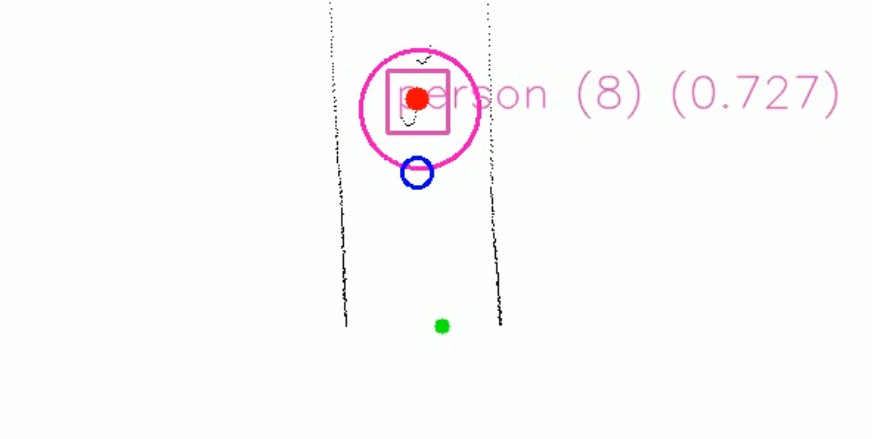
\includegraphics[width=100mm,clip]{figure/person_detector_laser_img2.png}
\caption{Automatic annotation overview}
\label{Generation of target coordinates}
\end{center}
\end{figure*}

\section{実験結果}

\begin{table}[tb]
    \begin{center}
      \caption{{Results of experiment}\label{Result}}
      \scalebox{1.5}[1.3]{
        \begin{tabular}{|c|r|} \hline
          Straight road & 100\% \\ \hline
          Curved road & 90\% \\ \hline
          Right angle road & 100\% \\ \hline
          Maximum tracking speed & 0.5 m/s \\ \hline
        \end{tabular}
      }
    \end{center}
\end{table}

直線経路、曲線経路、直角経路、最大追従速度の実験結果をFig. \ref{Result}に示す。
追従実験では、直線経路と直角経路がそれぞれ10回中10回成功した。曲線経路では、10回中9回成功した。
最大追従実験では、0.5[m/s]が最大追従速度となった。0.6[m/s]で3回実験したが、追従は確認されなかった。

\section{考察}
実験結果から直線経路と直角経路では、雑多な環境において一度も止まらず安定した挙動で要求仕様を
満たすことができた。しかし、曲線経路では一度だけ停止した。曲線経路で停止した原因は、ロボット用ノートPCのバッテリー低下だと考えられる。ロボットが停止しなかった場合のROS2 bagでは、システム全体の通信が平均10[Hz]以上で安定しているのに対し、曲線経路で停止したときは、平均4.9[Hz]であった。実験が成功しているROS2 bagでは、通信速度の低下は確認されず、ノートPCのバッテリーが10\%以下であったのは、曲線経路で停止した場合のみであった。